\section{Softwarearchitekture}

Die Software sollte nach dem Ports-and-Adapter Pattern 
\cite{cockburn2005hexagonal} aufgebaut sein, allerdings wurden nur 
Adapter implementiert. Nach einigen kleinen Änderungen wäre die 
Struktur wie folgt.

TODO Ist das so ok?

\begin{figure}[H]
    \begin{center}
        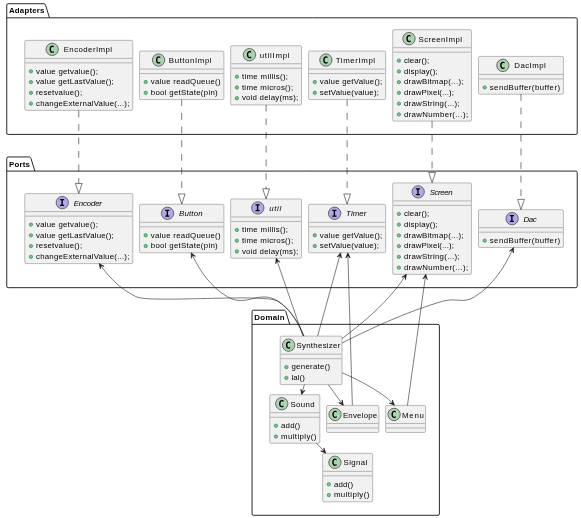
\includegraphics[width=\textwidth]{fig/UML_diagram.png}
    \end{center}
\end{figure}

\subsection{Adapter}

Porst bilden die Schnittstelle zur Hardware und zur ESP-IDF und 
Adapter ihre Implementierung.
Dadurch lässt sich der Kern unabhängig von diesen beiden Faktoren, also
auch auf einen normalen PC, testen. Im Folgenden werden alles Adapter und 
ihre Funktionen kurz erklärt.


\subsubsection{Digital-to-Analog Converter}
Die 
Kommunikation zwischen dem DAC und dem ESP32 findet über das I2S-Protokoll statt. Dazu wird die I2S-API der ESP-IDF
im Standard, TX und Mono-Modus verwendet.
Die 
Abtastrate und die Auflösung des 
Signals über eine Initialisierungsfunkion Übergeben.

The communication between the
DAC and the ESP32 happens via the I2S-protocol in standard, TX and mono mode
as described in the ESP-IDF-Documentation \cite{espidf2026api}. A signal can
be sent to the DAC by updating a buffer and calling the sendBuffer function 
with this buffer.

%blocking funktion

%tread save

%code example

%pictures

\subsubsection{User input}
The button Input can be read be calling button.getState\(Pin\) with the 
Pin-macro of the desired Pin. This returns weather or not the given pin is 
pulled low by pressing the button. The function readQueue will read from a
queue that contains the last 10 button presses. If it is used it should be
read accordingly often to avoid overfilling it. The debounstime for the 
buttons is 200ms.
% das ist sehr hoch vlt sollte ich da nochmal drüberschauen

A rotary encoder is used to edit numerical value. The encoder 
software-interface is implemented using the pulse-control-API as in
the ESP-IDF encoder example and contains two functions to interact with it. 
These are getValue and resetValue. getValue returns the current encoder value 
which can be incremented or decremented by turning the encoder. It goes to 
zero when reaching 256 or -256 or when calling resetValue.

\subsubsection{RGB-LED and LED}
An RGB-LED is used for...
%TODO

\subsubsection{Screen}
An I2C OLED-screen is integrated by using a library from voidlooprobotechs
github \cite{voidloop2026ssd1306}.
% schreiben falls ich die bib erweitere

\cite{espidf2026api}

TODO Timer, ThreadsaveVariable, Util

\subsection{Kern}

Der Kern der Anwendung besteht aus 3 Komponenten. Das sind die DSV-Bibliothek, welche
wie oben beschrieben, als eine Klasse namens Signal implementiert ist. Dann eine 
Erweiterung dieser Klasse namens Sound welche ein Audiosignal darstellt
und zuletzt die Synthesizer-Klasse, welche die Soundklasse nutzt, um mithilfe der 
Hardware einen Synthesizer zu implementieren. Diese 3 Komponenten werden in den 
folgenden Kapiteln beschrieben.
